\documentclass[journal=jacsat,manuscript=article]{achemso}
\usepackage[version=3]{mhchem} % Formula subscripts using \ce{}

\newcommand*\mycommand[1]{\texttt{\emph{#1}}}


\author{David J. Lary}
\affiliation{Hanson Center for Space Sciences, University of Texas at Dallas, Richardson TX 75080, USA}
\altaffiliation{Complex Exposure Threats Center Network (CETC), U.S. Department of Veterans Affairs}
\alsoaffiliation{ActivePure Technologies LLC, 14841 Dallas Pkwy #500, Dallas, TX 75254}
\email{David.Lary@utdallas.edu}
\author{John Waczak}
\affiliation{Hanson Center for Space Sciences, University of Texas at Dallas, Richardson TX 75080, USA}
\alsoaffiliation{ActivePure Technologies LLC, 14841 Dallas Pkwy #500, Dallas, TX 75254}
\author{John Sadler}
\affiliation{ActivePure Technologies LLC, 14841 Dallas Pkwy #500, Dallas, TX 75254}
\author{Joseph Urso}
\affiliation{ActivePure Technologies LLC, 14841 Dallas Pkwy #500, Dallas, TX 75254}
\author{Amy Carenza}
\affiliation{ActivePure Technologies LLC, 14841 Dallas Pkwy #500, Dallas, TX 75254}
\author{Andy Redmond}
\affiliation{ActivePure Technologies LLC, 14841 Dallas Pkwy #500, Dallas, TX 75254}
\author{Matthew D. Lary}
\affiliation{Hanson Center for Space Sciences, University of Texas at Dallas, Richardson TX 75080, USA}
\alsoaffiliation{ActivePure Technologies LLC, 14841 Dallas Pkwy #500, Dallas, TX 75254}

\title[An \textsf{achemso} demo]
  {HEART: \underline{H}olistic \underline{E}nvironmental \underline{A}erosol and \underline{R}eactive Component \underline{T}esting}

\abbreviations{IR,NMR,UV}
\keywords{American Chemical Society, \LaTeX}

\begin{document}

\begin{tocentry}

Some journals require a graphical entry for the Table of Contents.
This should be laid out ``print ready'' so that the sizing of the
text is correct.

Inside the \texttt{tocentry} environment, the font used is Helvetica
8\,pt, as required by \emph{Journal of the American Chemical
Society}.

The surrounding frame is 9\,cm by 3.5\,cm, which is the maximum
permitted for  \emph{Journal of the American Chemical Society}
graphical table of content entries. The box will not resize if the
content is too big: instead it will overflow the edge of the box.

This box and the associated title will always be printed on a
separate page at the end of the document.

\end{tocentry}

\begin{abstract}
    The COVID-19 pandemic highlighted the importance of characterizing indoor air quality (iAQ) for human health. Due to the enormous variety of air quality components (airborne aerosols, bio-aerosols, gases, ions) together with the need to characterize the wavelength-resolved light intensity driving indoor photochemistry, this is a challenging task to do well. Indoor air typically contains thousands of distinct VOCs. Historically, simply increasing the ventilation rate has been the go-to method for improving indoor air quality. However, this increases energy consumption (and associated greenhouse gas emissions). Further, if downwind of pollution sources (e.g. forest fires or heavy traffic), bringing in outside air can degrade iAQ. It is therefore timely to improve iAQ observation and simulation for health applications. This study presents a holistic approach for indoor air quality observations, simulation, and data assimilation called HEART (\underline{H}olistic \underline{E}nvironmental \underline{A}erosol and \underline{R}eactive Component \underline{T}esting). Chemical data assimilation coupled with direct observations allows inference of critical unobserved radicals such as OH (with an uncertainty estimate) and ions, which are typically hard to observe. As UV lamps and photocatalytic oxidation become more widely used, in addition to HEPPA filtration and variable air change rates, this approach becomes of greater utility.
\end{abstract}

\section{Introduction}
There has never been a more pressing need to accurately and comprehensively observe and simulate indoor air quality for public health applications. This is particularly relevant  in the wake of the global COVID-19 pandemic when considering guidelines for minimum ventilation rates and other strategies to improve indoor air quality (iAQ) so that it is optimal for human occupants and minimizes adverse health effects.

The COVID-19 pandemic that occurred globally between March 11, 2020 and May 5, 2023, resulted in more than 550 million confirmed cases of COVID-19 and over 6.3 million fatalities worldwide. This event has underscored the crucial significance of indoor air quality for human \hbox{health \citep{who_pandemic}}. The quality of indoor air has a significant effect on physical health, cognitive performance, and general well-being \citep{Krebs2021AirPC, Gao2021ShorttermAP, Carneiro2021TheEO, Ni2021AssociationsOP, Shehab2019EffectsOS}. According to the World Health Organization (WHO), 3.2 million people die prematurely each year from illnesses attributable to indoor air pollution \citep{who2021indoor}, indoor air pollution is responsible for approximately 4.1\% of global deaths. 

According to the National Human Activity Pattern Survey (NHAPS), prior to COVID, Americans spent up to 90\% of their time indoors \citep{klepeis2001}.  The amount of time a given individual spends indoors varies depending on lifestyle, profession, geographical location, cultural habits, and personal health. The advent of the Internet, digital entertainment, and remote work options has further increased the amount of time many people spend indoors. The widespread use of computers, smartphones, and other devices has allowed one to work, socialize, and participate in various leisure activities without leaving the comfort of indoor spaces.  The COVID-19 pandemic had a profound impact globally on how people lived their life, especially how much time they spent indoors. People in the United States, for example, spent an additional 10 hours per week indoors during the pandemic than they did before the pandemic \citep{oxford_study}. This rise in indoor time was caused by a number of factors, including social distancing rules, school closures, and work-from-home policies.

The Centers for Disease Control and Prevention (CDC) found that indoor transmission of COVID-19 is far more likely than outdoor transmission, with 90\% of COVID-19 infections occurring indoors \citep{cdc_indoor_transmission}. Similarly, because virus transmission occurs through respiratory droplets created when an infected person coughs or sneezes, the risk of catching \hbox{COVID-19} indoors is 20 times greater than the risk of contracting it outdoors \citep{ucsf_indoor_transmission}. Small respiratory droplets (bio-aerosols) can linger in indoor air for hours and subsequently be inhaled by those nearby. 

\subsection{Attention to the Details: More Than Just Passive Filtration}

Comprehensively and accurately characterizing the composition of indoor air for human health studies is a significant (if not daunting) undertaking due to the large number and variety of air quality components, including airborne aerosols, bio-aerosols, gases, and ions. Furthermore, it is a challenging task because of the sheer diversity of environmental settings, pollution sources, and the varying characteristics that define different interior spaces. Just the gaseous composition of indoor air can involve thousands of different volatile organic compounds (VOCs) \citep{shin2020, choi2016}.

For quite some time, simply increasing the ventilation rate, and bringing in \lq clean' outside air has been the go-to method for improving indoor air quality \citep{drees1992ventilation, Burton1993ASHRAEsIA, Mendell2014BalancingEC, Dutton2015EvaluationOT, Johnson2018IndoorAQ, Lohani2016SmartVentAC, Zhang2022ARO}. Nevertheless, this results in an escalation in energy consumption, leading to higher costs and any associated emission of greenhouse gases from electrical power generation. Furthermore, what happens if there is a pollution event in the outdoor air, such as caused by being downwind of a forest fire or heavy traffic? Under these conditions bringing in outside air will negatively impact the indoor air quality. 

As airborne transmission became the clear mechanism of SARS-CoV-2 spread, multiple studies confirmed that in some cases there can be negative consequences of high air change rates. One study observed that when the air changes per hour (ACH) was increased from 1.8 to 12, the time to peak virus concentration in connected rooms decreased from 30 minutes to 11 \cite{pease_investigation_2021}. A separate contact-tracing case study found that six students were infected by a teacher in a distant room, despite the use of high-efficiency particulate air filters throughout the building \cite{turakhia_ultrafast_2021}. Indeed, amidst observations of increased HVAC energy consumption by upwards of 128\% in one Chinese district, researchers still concluded that “HVAC systems may turn out to be the culprit of microbial contamination in enclosed spaces and deteriorate the environment due to inappropriate design and operation”  \cite{zheng_covid-19_2021}.

While altering the ventilation rate is clearly helpful for treating stale air and minimizing so-called sick-building syndrome, it falls short when dealing with pollutants (such as VOCs) and airborne viruses. When it comes to improving indoor air quality, the real challenges given by global environmental change, together with growing utility prices due to inflation and geopolitical shocks to energy supply chains, have produced an implicit dichotomy between sustainability and public health goals. 

It is not just health outcomes that are associated with poor air quality. Numerous studies have demonstrated that poor air quality diminishes both human cognitive and physical performance \citep{Krebs2021AirPC, Gao2021ShorttermAP, Carneiro2021TheEO, Ni2021AssociationsOP, Shehab2019EffectsOS}. Degraded cognitive performance has a significant impact on society, ranging from poor learning outcomes in schools to impaired decision-making performance and productivity at work. As a result, the ability to adequately and comprehensively quantify the performance of indoor air quality remediation systems is critical for guiding appropriate, science-based threat mitigation strategies. If HVAC control is driven by an incomplete subset of metrics/contaminants of concern, buildings will clearly fail to adapt to unexpected threats. For instance, CO$_2$ is frequently used as a control metric because it acts as a tracer gas to control the ventilation rate per person by controlling the indoor/outdoor differential. However, using CO$_2$ along with other metrics is beneficial. For example, five studies found that CO$_2$ control alone cannot control for pollutants generated outdoors or indoors independent of human activity \cite{zaatari_impact_2016}. More recently, one COVID-19 case study discovered that the rapid spread of the disease through a nursing home ward was most likely caused by decreased ventilation by a CO$_2$ demand control ventilation system optimized solely for decreased energy-demand \cite{lamping_air_nodate}.

\subsection{Active Filtration Systems}

To rise to this challenge we need to pay careful attention to the details in at least two key areas. First, to create high-iAQ, low-energy, climate-resilient buildings for the future, we need to embrace alternatives to solely relying on outside air ventilation to maintain healthy indoor environments, thereby building on key lessons from the COVID-19 pandemic about layered air cleaning strategies \citep{enVeridWhitePaper}. Second, comprehensively characterizing the chemistry of iAQ becomes imperative if the layered air cleaning strategies  involve components such as UV lamps \citep{peng2023significant, Denny2010IntegratedPF, Nitter2019UVTA, Peng2023SignificantPO} or photocatalytic oxidation \citep{Lorencik2015IndoorAQ, Mata2022IndoorAQ, Nath2014PHOTOCATALYTICOO}.

In the global outdoor environment, sunlight incident on the Earth's atmosphere is the ultimate driving force of a host of photo-chemical and environmental processes (e.g. photosynthesis, photolysis, atmospheric radiative heating). Accurately characterizing atmospheric radiative transfer plays a key role in modeling outdoor atmospheric chemistry and the weather/climate system \cite{Chandrasekhar1960, Lenoble1985, Lary1991a, Lary1991b, Deutschmann:2011, Hartmann:2016, Buehler:2017, Zhang:2019}. Likewise, light is a key driver for iAQ, particularly when this involves the high-energy photons associated with the ultraviolet wavelengths (\hbox{10--400 nm}, with \hbox{UV-A 315--400 nm}, \hbox{UV-B 280--315 nm}, or \hbox{UV-C 100--280 nm}). Photolysis is a critical facet for indoor air quality \citep{carslaw2007} which is all too often overlooked.

\subsection{Photochemical Cascades and Secondary Organic Aerosols}

Unlike passive systems, active systems neutralize pathogens while they are still in the air. It is therefore imperative that when such active systems are deployed the detailed impacts on iAQ are fully characterized \citep{Joo:2021}. It is clearly time for a strategy that goes well beyond just six criterion air pollutants.

The photolysis of gases, such as, for example,  O$_2$, H$_2$O, and O$_3$, leads to the production of highly reactive free radical oxidizing agents such O($^1$D), O($^3$P), and OH and the resultant initiation of large photochemical reaction cascades that can have a significant impact on iAQ. Further, if nitrogen oxides are present, then oxidizing agents such as NO$_3$ will also be produced by photolysis. Likewise, if halogens are present, such as due to the use of cleaning products involving bleach, then oxidizing agents such as Cl will also be produced by photolysis. Each of these oxidizing agents can play a significant role in iAQ. The precise impact is a sensitive function of the local physical (temperature, pressure, illumination, surface charge distributions, and the type and area of surfaces available for heterogeneous reactions) and the chemical environment. Given that thousands of VOCs can be present in iAQ we begin to see just how daunting comprehensively characterizing iAQ becomes.  

Further, the oxidation of VOCs can lead to the formation of secondary organic aerosols \citep{Joo:2021, Claeys2004FormationOS, Srivastava2022FormationOS, Fan2022ARO}, typically ranging in size from 0.1 to 1 $\mu$m. The size of aerosols determines their depth of penetration into the human respiratory tract and lungs. Generally, larger particles tend to deposit in the upper airways (nasal cavity, pharynx, larynx), while smaller particles have a greater likelihood of reaching the lower airways (trachea, bronchi, bronchioles, alveoli). Coarse particles (particles with aerodynamic diameters between 2.5 to 10 $\mu$m) primarily deposit in the upper airways, with limited penetration into the lower airways. Fine particles (particles with aerodynamic diameters between 0.1 and 2.5 $\mu$m) can penetrate deeper into the respiratory tract, with a significant portion reaching the lower airways, including bronchi and bronchioles. Ultrafine particles (particles with aerodynamic diameters less than 0.1 $\mu$m), such as SOA, have high potential for deep penetration into the lower airways and alveolar region of the lungs.

\section{Materials and Methods}

\subsection{HEART Sensing System}

\begin{figure}[t!]
  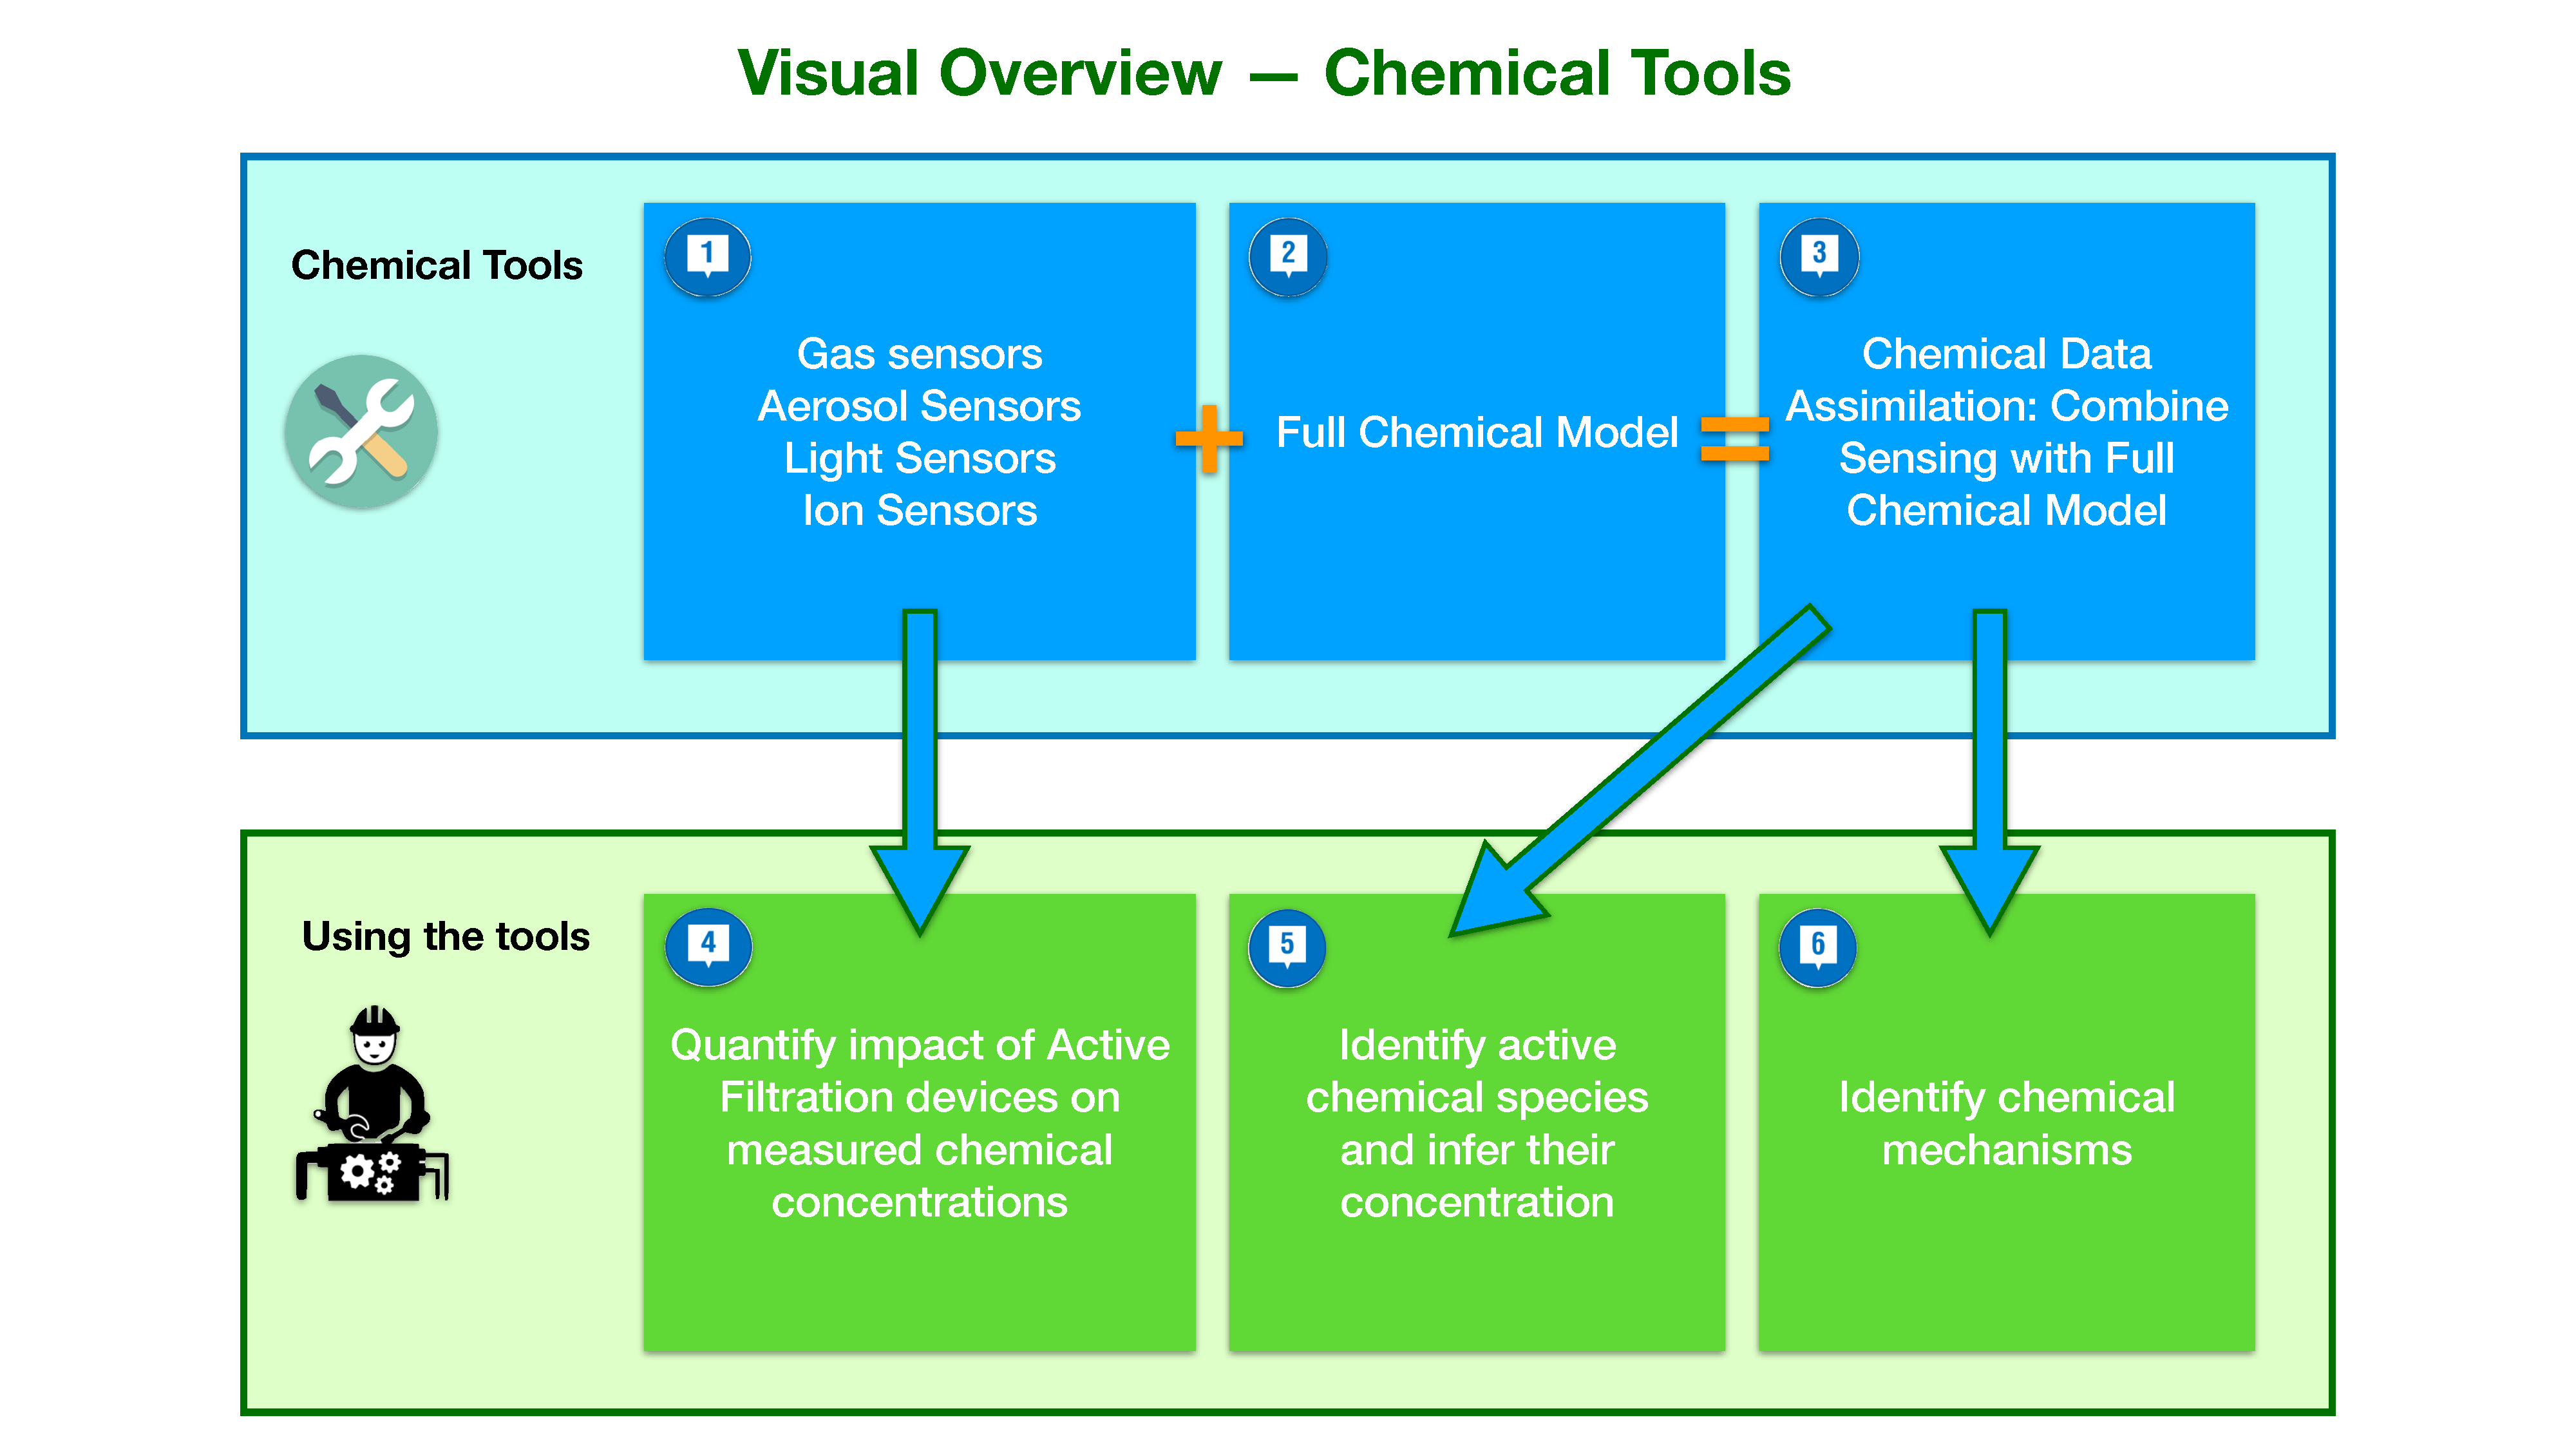
\includegraphics[width=\textwidth]{Figures/ChemicalTools.pdf}
  \vspace{-0.2in}
  \caption{A schematic representation of the HEART (\underline{H}olistic \underline{E}nvironmental \underline{A}erosol and \underline{R}eactive Component \underline{T}esting) iAQ suite of tools described in this study.}
  \label{Figure:ChemicalTools}
\end{figure}


Given the current scale of the challenges to human health and well-being associated with iAQ, it is timely to holistically  characterize as many aspects of iAQ as possible in the built environment. This study introduces the HEART (\underline{H}olistic \underline{E}nvironmental \underline{A}erosol and \underline{R}eactive Component \underline{T}esting) suite. HEART is designed for the comprehensive characterization of air quality including the chemical composition (characterizing hundreds of chemicals), positive and negative ion densities, aerosol size (from 5 nm to 100 microns), aerosol morphology (shape), aerosol composition, and individual bio-aerosol particle recognition, along with the accurately characterized illumination environment characterized for more than 4,000 wavelength intervals from the UV to the near-infrared (\hbox{190 — 1,100 nm}) using a NIST calibrated spectrometer. The lighting environment is important, as, after all, air quality is atmospheric photochemistry in the indoor built environment, and photolysis is a key driver. Furthermore, some of the frequently advocated families of technologies make use of various parts of the ultraviolet spectrum. This high-energy region of the spectrum has important implications for indoor air quality.

\subsection{Photochemical Modelling System}

\subsection{Uncertainty Estimation}

\subsection{Photochemical Data Assimilation System}




\section{Results and discussion}

\subsection{Outline}

The document layout should follow the style of the journal concerned.
Where appropriate, sections and subsections should be added in the
normal way. If the class options are set correctly, warnings will be
given if these should not be present.

\subsection{References}

The class makes various changes to the way that references are
handled.  The class loads \textsf{natbib}, and also the
appropriate bibliography style.  References can be made using
the normal method; the citation should be placed before any
punctuation, as the class will move it if using a superscript
citation style
\cite{Mena2000,Abernethy2003,Friedman-Hill2003,EuropeanCommission2008}.
The use of \textsf{natbib} allows the use of the various citation
commands of that package: \citeauthor{Abernethy2003} have shown
something, in \citeyear{Cotton1999}, or as given by
Ref.~\citenum{Mena2000}.  Long lists of authors will be
automatically truncated in most article formats, but not in
supplementary information or reviews \cite{Pople2003}. If you
encounter problems with the citation macros, please check that
your copy of \textsf{natbib} is up to date. The demonstration
database file \texttt{achemso-demo.bib} shows how to complete
entries correctly. Notice that ``\latin{et al.}'' is auto-formatted
using the \texttt{\textbackslash latin} command.

Multiple citations to be combined into a list can be given as
a single citation.  This uses the \textsf{mciteplus} package
\cite{Johnson1972,*Arduengo1992,*Eisenstein2005,*Arduengo1994}.
Citations other than the first of the list should be indicated
with a star. If the \textsf{mciteplus} package is not installed,
the standard bibliography tools will still work but starred
references will be ignored. Individual references can be referred
to using \texttt{\textbackslash mciteSubRef}:
``ref.~\mciteSubRef{Eisenstein2005}''.

The class also handles notes to be added to the bibliography.  These
should be given in place in the document \bibnote{This is a note.
The text will be moved the the references section.  The title of the
section will change to ``Notes and References''.}.  As with
citations, the text should be placed before punctuation.  A note is
also generated if a citation has an optional note.  This assumes that
the whole work has already been cited: odd numbering will result if
this is not the case \cite[p.~1]{Cotton1999}.

\subsection{Floats}

New float types are automatically set up by the class file.  The
means graphics are included as follows (Scheme~\ref{sch:example}).  As
illustrated, the float is ``here'' if possible.
\begin{scheme}
  Your scheme graphic would go here: \texttt{.eps} format\\
  for \LaTeX\, or \texttt{.pdf} (or \texttt{.png}) for pdf\LaTeX\\
  \textsc{ChemDraw} files are best saved as \texttt{.eps} files:\\
  these can be scaled without loss of quality, and can be\\
  converted to \texttt{.pdf} files easily using \texttt{eps2pdf}.\\
  %\includegraphics{graphic}
  \caption{An example scheme}
  \label{sch:example}
\end{scheme}

\begin{figure}
  As well as the standard float types \texttt{table}\\
  and \texttt{figure}, the class also recognises\\
  \texttt{scheme}, \texttt{chart} and \texttt{graph}.
  \caption{An example figure}
  \label{fgr:example}
\end{figure}

Charts, figures and schemes do not necessarily have to be labelled or
captioned.  However, tables should always have a title. It is
possible to include a number and label for a graphic without any
title, using an empty argument to the \texttt{\textbackslash caption}
macro.

The use of the different floating environments is not required, but
it is intended to make document preparation easier for authors. In
general, you should place your graphics where they make logical
sense; the production process will move them if needed.

\subsection{Math(s)}

The \textsf{achemso} class does not load any particular additional
support for mathematics.  If packages such as \textsf{amsmath} are
required, they should be loaded in the preamble.  However,
the basic \LaTeX\ math(s) input should work correctly without
this.  Some inline material \( y = mx + c \) or $ 1 + 1 = 2 $
followed by some display. \[ A = \pi r^2 \]

It is possible to label equations in the usual way (Eq.~\ref{eqn:example}).
\begin{equation}
  \frac{\mathrm{d}}{\mathrm{d}x} \, r^2 = 2r \label{eqn:example}
\end{equation}
This can also be used to have equations containing graphical
content. To align the equation number with the middle of the graphic,
rather than the bottom, a minipage may be used.
\begin{equation}
  \begin{minipage}[c]{0.80\linewidth}
    \centering
    As illustrated here, the width of \\
    the minipage needs to allow some  \\
    space for the number to fit in to.
    %\includegraphics{graphic}
  \end{minipage}
  \label{eqn:graphic}
\end{equation}

\section{Experimental}

The usual experimental details should appear here.  This could
include a table, which can be referenced as Table~\ref{tbl:example}.
Notice that the caption is positioned at the top of the table.
\begin{table}
  \caption{An example table}
  \label{tbl:example}
  \begin{tabular}{ll}
    \hline
    Header one  & Header two  \\
    \hline
    Entry one   & Entry two   \\
    Entry three & Entry four  \\
    Entry five  & Entry five  \\
    Entry seven & Entry eight \\
    \hline
  \end{tabular}
\end{table}

Adding notes to tables can be complicated.  Perhaps the easiest
method is to generate these using the basic
\texttt{\textbackslash textsuperscript} and
\texttt{\textbackslash emph} macros, as illustrated (Table~\ref{tbl:notes}).
\begin{table}
  \caption{A table with notes}
  \label{tbl:notes}
  \begin{tabular}{ll}
    \hline
    Header one                            & Header two \\
    \hline
    Entry one\textsuperscript{\emph{a}}   & Entry two  \\
    Entry three\textsuperscript{\emph{b}} & Entry four \\
    \hline
  \end{tabular}

  \textsuperscript{\emph{a}} Some text;
  \textsuperscript{\emph{b}} Some more text.
\end{table}

The example file also loads the optional \textsf{mhchem} package, so
that formulas are easy to input: \texttt{\textbackslash ce\{H2SO4\}}
gives \ce{H2SO4}.  See the use in the bibliography file (when using
titles in the references section).

The use of new commands should be limited to simple things which will
not interfere with the production process.  For example,
\texttt{\textbackslash mycommand} has been defined in this example,
to give italic, mono-spaced text: \mycommand{some text}.

\section{Extra information when writing JACS Communications}

When producing communications for \emph{J.~Am.\ Chem.\ Soc.}, the
class will automatically lay the text out in the style of the
journal. This gives a guide to the length of text that can be
accommodated in such a publication. There are some points to bear in
mind when preparing a JACS Communication in this way.  The layout
produced here is a \emph{model} for the published result, and the
outcome should be taken as a \emph{guide} to the final length. The
spacing and sizing of graphical content is an area where there is
some flexibility in the process.  You should not worry about the
space before and after graphics, which is set to give a guide to the
published size. This is very dependant on the final published layout.

You should be able to use the same source to produce a JACS
Communication and a normal article.  For example, this demonstration
file will work with both \texttt{type=article} and
\texttt{type=communication}. Sections and any abstract are
automatically ignored, although you will get warnings to this effect.

%%%%%%%%%%%%%%%%%%%%%%%%%%%%%%%%%%%%%%%%%%%%%%%%%%%%%%%%%%%%%%%%%%%%%
%% The "Acknowledgement" section can be given in all manuscript
%% classes.  This should be given within the "acknowledgement"
%% environment, which will make the correct section or running title.
%%%%%%%%%%%%%%%%%%%%%%%%%%%%%%%%%%%%%%%%%%%%%%%%%%%%%%%%%%%%%%%%%%%%%
\begin{acknowledgement}

Please use ``The authors thank \ldots'' rather than ``The
authors would like to thank \ldots''.

The author thanks Mats Dahlgren for version one of \textsf{achemso},
and Donald Arseneau for the code taken from \textsf{cite} to move
citations after punctuation. Many users have provided feedback on the
class, which is reflected in all of the different demonstrations
shown in this document.

\end{acknowledgement}

%%%%%%%%%%%%%%%%%%%%%%%%%%%%%%%%%%%%%%%%%%%%%%%%%%%%%%%%%%%%%%%%%%%%%
%% The same is true for Supporting Information, which should use the
%% suppinfo environment.
%%%%%%%%%%%%%%%%%%%%%%%%%%%%%%%%%%%%%%%%%%%%%%%%%%%%%%%%%%%%%%%%%%%%%
\begin{suppinfo}

This will usually read something like: ``Experimental procedures and
characterization data for all new compounds. The class will
automatically add a sentence pointing to the information on-line:

\end{suppinfo}

%%%%%%%%%%%%%%%%%%%%%%%%%%%%%%%%%%%%%%%%%%%%%%%%%%%%%%%%%%%%%%%%%%%%%
%% The appropriate \bibliography command should be placed here.
%% Notice that the class file automatically sets \bibliographystyle
%% and also names the section correctly.
%%%%%%%%%%%%%%%%%%%%%%%%%%%%%%%%%%%%%%%%%%%%%%%%%%%%%%%%%%%%%%%%%%%%%
\bibliography{references.bib}

\end{document}